\chapter{Background}
\label{ch2}
\Fors{T} relies on the research from many fields of study in both mathematics and computer science. In this chapter we will briefly examine the underlying theory, concepts, and frameworks upon which we rely to convey the ideas presented in this thesis and bring to fruition the work invested in designing and developing \Fors{t}.
\todoReword{Elaborate like a teasing summary}

%
%
%
%
\section{Basic Theory}\todoReword{theoretical foundation}
The following is an abbreviated list of the important theoretical concepts used in the chapters to follow. These include concepts from set theory, geometry, and topology.

%
%
\subsection{Set Theory}
A set is one of the most fundamental concepts in mathematics. Informally, a set is a collection of distinct objects, and is also itself considered to be an object. In this thesis, sets are denoted using capital, calligraphic letters, such as: $\bM$, $\bP$, $\bT$, and $\bF$.

%
\subsubsection{Set Definitions}
A set may be defined using ``intensional definitions'' or ``extensional definitions''. An intensional definition uses semantic rules and symbols, where each symbol can be translated into words so that the definition may be coherently read aloud. For example:
%
\begin{equation}
	\bP := \left \{\:\bp_v \mid v \in \mathbb{N}, \;\text{and}\; 1\leq v \leq v_{max}\:\right \}
\end{equation}
%
which should be read as, ``$\bP$ is defined as the set of all points $\bp_v$, such that the index $v$ is a member of the set of natural numbers, and $v$ is a number from 1 to the maximum index of points in the set.''

The other option, extensional definition, is denoted by enclosing the list of members in curly brackets, and optionally invoking an ellipsis (``\dots'') for continuing into infinity. For example:
%
\begin{equation}
	\mathbb{N} = \left \{\:0,\,1,\,2,\,3,\,\ldots\:\right \}
\end{equation}
%
A set member is allowed to be listed two or more times in a definition, for example $\left \{\:4,\,2,\,2\:\right \}$. However, it is identical to the set $\left \{\:4,\,2\:\right \}$ per the axiom of extensionality\todoResearch{Zermelo–Fraenkel set theory., Axiom of extensionality, logical extensionality}, which states that two definitions of sets, which differ only in that one of the definitions lists members multiple times, define the same set.

%
\subsubsection{Special Sets}
There exists some sets which are used in mathematical literature with such frequency as to demand their own standardized symbols. In this thesis\todoReference{defineSetofNaturalNumbers}, we have already encountered $\mathbb{N}$, which denotes the set of all natural numbers.

%
\subsubsection{Cardinality}
Denoted as $|\bM\,|$, the cardinality of a set is the number of its members, so if $\bM = \left \{\,\bP,\,\bT\right \}$, then $|\bM\,| = 2$.

%
\subsubsection{Membership \& Relational Operators}
If an object is said to be a member of a set, it is written with the symbol $\in$ and expressed as either belonging to or being an element of the set. Similarly, a set may be the subset of another set, written with the symbol $\subseteq$, meaning that every member of the first set is also a member of second set. A superset works exactly in reverse, written with the symbol $\subseteq$, it is the identity where every member of the second set is also a member of first set. In mathematical notation, those examples are written as\footnote{The negative operators also exists as $\notin$ and $\nsubseteq$}
\begin{align}
	B & \in \left \{A,\,B,\,C\right \} \\
	\left \{A,\,B\right \} & \subseteq \left \{A,\,B,\,C\right \} \\
	\left \{A,\,B,\,C\right \} & \supseteq \left \{A,\,B\right \}
\end{align}

%
\subsubsection{Binary Operations}
Among all the basic binary operations one can perform on a set\footnote{which are the union, intersection, complement, and Cartesian product}, in this thesis, we exclusively use the union operation, denoted as $\cup$, whose output is the set of all objects that are members of either set, or both. For example:
\begin{equation}
	\left \{0,\,1,\,2\right \} \cup \left \{2,\,3,\,4\right \} = \left \{0,\,1,\,2,\,3,\,4\right \}
\end{equation}
\todoReword{would look better to have words here}
Also importantly, as in addition of scalar values, the associative property for a union of sets says that how the sets are grouped does not change the result.\todoCitation{associate property of unions}

As a final note, a ``family of sets'' is very similar to a superset, with only the subtle difference that all the subsets it contains should have some quality in common. For example, in Section~\ref{ch2s3ssNRN} we will define the set of sets of neighbors as a family of sets, with the common quality being that all the subsets are neighborhoods.

%
%
%
\subsection{Linear Algebra}
\label{ch2sBssLA}
Nearly as fundamental as set theory, linear algebra is the branch of mathematics which studies the different methods and representations which may concern a line, including: sets of equations, matrices, transformations, vector spaces, norming functions, etc. It is used in almost all scientific domains that use mathematics, including geometry and scientific computing, as well as provides the symbols and concepts for performing blocks of operations in parallel.~\cite{Weisstein19i} \todoCitation{position vector}

%
\subsubsection{Position Vectors}
\label{ch2sBssLAsssPV}
A position vector is represented by a set of Cartesian coordinates with cardinality matching that of the dimensionality of the Euclidean space in which it is embedded. For example, in Section~\ref{ch2s3ssP}\todoReword{add back reference for this section} we say that a point can also be called a position vector, so if we are given a point in $\bR{3}$, it is defined by the three Cartesian coordinates $x$, $y$, and $z$. ``Cartesian'' refers to the French scholar René Descartes~\cite{EB1}, and ``Euclidean'' refers to Euclid of Alexandria, the Ancient Greek mathematician~\cite{EB2}.

Figure~\ref{fig:definePositionVector} provides three examples of why a point may be called a position vector. Any set of coordinates have an implied direction pointing away from the origin, which in $\bR{3}$ is located at $(0, 0, 0)$. In (a) the point $\bp_a$ is in $\bR{1}$ and located at at coordinate $(4)$ which is at a distance of $4$ units away from the origin. In (b) the point $\bp_b$ is in $\bR{2}$ and located at at coordinates $(4,\,4)$ which is at a distance of $4\sqrt{2}$ units away from the origin. In (c) the point $\bp_c$ is in $\bR{3}$ and located at at coordinates $(4,\,4,\,4)$ which is at a distance of $4\sqrt{3}$ units away from the origin. This concept extends to any Euclidean space $\bR{n}$.

\begin{figure}[ht]
\ffigbox
	{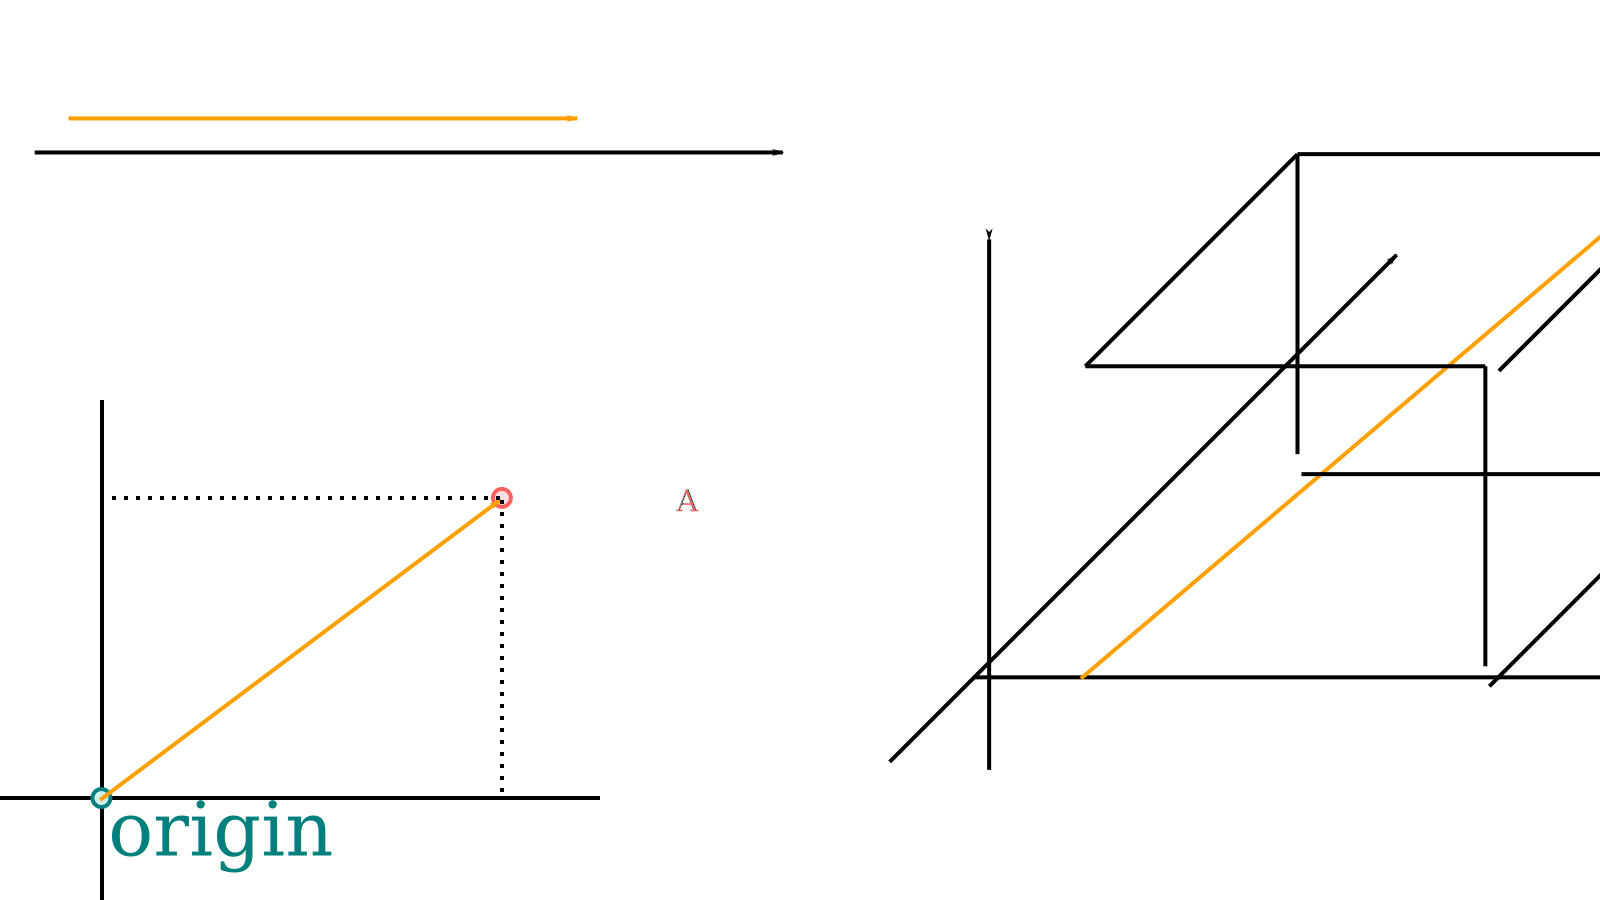
\includegraphics[width=1.0\linewidth]{figures/definePositionVector.png}}
	{\caption[Examples of Position Vector]{Three examples of position vectors shown as arrows in sand color pointed from the origin in teal color to the points in coral color: (a) $\bp_a$ in $\bR{1}$ at coordinate $(4)$ with length 4, (b) $\bp_b$ in $\bR{2}$ at coordinates $(4,\,4)$ with length $4\sqrt{2}$, (c) $\bp_c$ in $\bR{3}$ at coordinates $(4,\,4,\,4)$ with length $4\sqrt{3}$. The origins are located at $(0)$, $(0,\,0)$, and $(0,\,0,\,0)$ respectively.}\label{fig:definePositionVector}}
\end{figure}

%
\subsubsection{Subtracting Two Vectors}
\label{ch2sBssLAsssS2V}
Among the binary operators with which one could operate on vectors, this thesis is primarily concerned with subtraction. In order to perform subtract of two vectors in the same Euclidean space, one must simply subtract each component element-wise.\~cite{Weisstein19j} For example, given two points in $\bR{3}$, $A$ and $B$
\todoBackground{vector subtraction}
\begin{equation}
	A - B = (A_x - B_x, A_y - B_y, A_z - B_z)
	\label{eq:vectorSubtraction}
\end{equation}

%
\subsubsection{L2-norm}
\label{ch2sBssLAsssL2N}
The L2-norm may be seen abbreviated as $L^2$ or $\ell^2$, or perhaps called the ``Euclidean norm'' or ``Euclidean distance'' elsewhere in the literature. It is so named because it is the ordinary, straight line distance between two points in Euclidean space, and in the case of a position vector in $\bR{3}$, the two points are the origin at $(0, 0, 0)$ and $\bp$.~\cite{Weisstein19h}\todoBackground{find all L2-norm and edge length references, and introduce the concept here}

The purpose for calculating the L2-norm of a vector is to determine the ordinary, single-dimension length of the vector, regardless of the dimensionality of Euclidean space in which it is embedded. For three examples, see in Figure~\ref{fig:definePositionVector} how despite having all coordinates exclusively set to $4$, the position vector on (a) is of length $4$, in (b) it is of length $4\sqrt{2} \approx 5.657$, and in (c) it is of length $4\sqrt{3} \approx 6.928$.

To determine the length of a vector, one can use the equation for the L2-norm
\begin{equation}
	|\bp| \enspace=\enspace \|\bp\|_2 \enspace=\enspace \sqrt{x^2 + y^2 + z^2 + \ldots + n^2} \enspace:\enspace \bp \in \bR{n}
	\label{eq:l2norm}
\end{equation}

In this thesis, the L2-norm is denoted using the symbols $\|\bp\|_2$, or abbreviated as $|\bp|$. Please note the similar notation for the cardinality of a set $|\bP|$. While the matching symbols do represent somewhat similar concepts, cardinality is the count of elements in the set, but the L2-norm of a vector is calculated as in Equation~\ref{eq:l2norm}.~\cite[p.~26]{Mara12}

%
%
%
\subsection{Geometry}
As vast and encompassing is geometry as a field of study, of paramount importance for \fors{t} are interpolation, the concept of a geodesic disc, and the characteristics of a circle sector.
\todoResearch{weighted averaging using density}

%
\subsubsection{Interpolation \& Extrapolation}
\todoBackground{add text and figure for extrapolation}
Simply stated, interpolation is a method of constructing new data points within the range of a discrete set of known data points, such as those points used in \tdd{}. There exist a large variety of methods for interpolating different kinds of data\todoCitation{different kinds of interpolation}, but as an introduction, let us first consider linear interpolation, which is simple to calculate\footnote{however can become imprecise in relation to the square of the distance between the data points.}\todoCitation{footnote:error of linear interpolation} and can be extended for n-dimensions\todoCitation{n-dimensional linear interpolation}.

Given the two data points in $\bR{2}$, $(x_a, y_a)$ and $(x_b, y_b)$, the so called interpolant of a point located at\todoReword{interpolant is wrong, don't use point located at, maybe value sampled at instead?} $x_c$ can be calculated as
%
\begin{equation}
	y_c = y_a + (y_b - y_a) \frac{x_c - x_a}{x_b - x_a}
	\label{eq:interpolationGeneral}
\end{equation}

To illustrate the concept of interpolation, consider the two points $(1, 2)$ and $(5, 1)$, then find the $y$ value of a point located along the line $x = 3$
%
\begin{align}
	y_c & = 2 + (1 - 2) \frac{3 - 1}{5 - 1} \\
	& = 2 + -1 \frac{2}{4} \enspace = \enspace  1.5
	\label{eq:interpolationSpecific}
\end{align}

So the value halfway between the two given points is interpolated to be $(2,\,2.5)$, which is halfway between as expected. Interpolation becomes even more intuitive when seen graphically as shown in Figure~\ref{fig:interpolation}.

\begin{figure}
\ffigbox
	{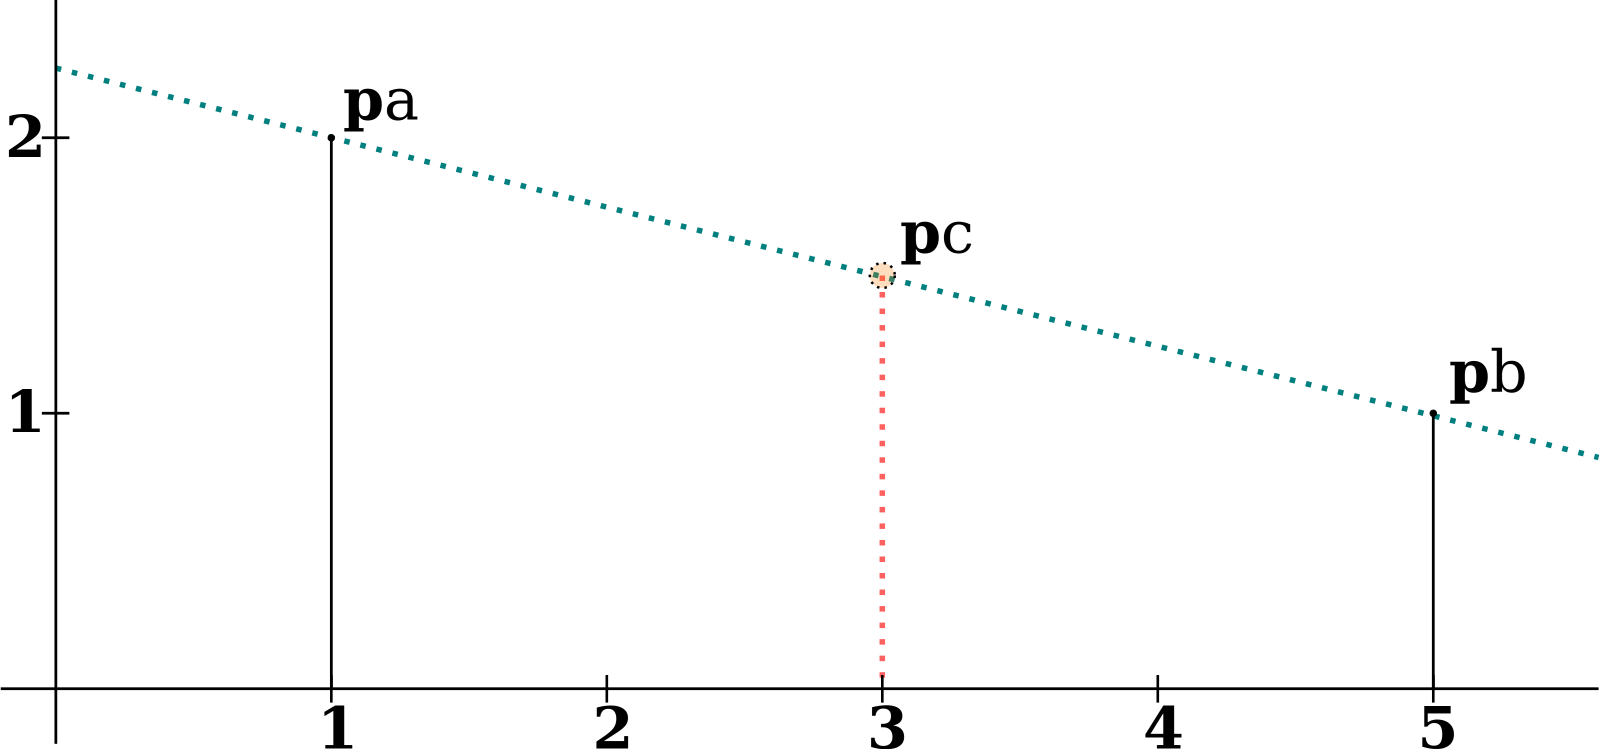
\includegraphics[width=1.0\linewidth]{figures/interpolation.png}}
	{\caption[Interpolation between two points in $\bR{2}$]{$\bp_c$ is interpolated as a value between $\bp_a$ and $\bp_b$}\label{fig:interpolation}}
\end{figure}

%
\subsubsection{Geodesic Discs}
\label{ch2sBssGsssGD}
\todoResearch{geodesic discs}
Geodesic Disc $\bO$%
\nomenclature[aa]{$\bO$}{a geodesic disc}%
\nomenclature[ab]{$\bO_v$}{a specific geodesic disc centered about the point $\bp_v$}%

%
\subsubsection{Circle Sectors}
\label{ch2sBssGsssCS}
A circular sector, or circle sector, is the portion of a disc enclosed by two radii and an arc. In general, the larger area is known as the major sector, however \fors{t} is only concerned with the area of the other, smaller area, known as the minor sector. Going forward, the minor circle sector will be abbreviated as just the circle sector, or even more simply, the sector. In general, we will denoted sectors as $\bs$, or $bs_i$ in reference to a specific circle sector in a geodesic disc $\bO$.%
\nomenclature[ba]{``the sector''}{or the circle sector; the minor sector of a circle defined by its radius and central angle}%
\nomenclature[bb]{$\bs$}{a circle sector}%
\nomenclature[bc]{$\bs_i$}{specific circle sector in a specific geodesic disc $\bO$}%

As the sector can be described entirely by the central angle $\alpha$ and the circle's radius $\ell_{a,b}$, the area of the sector can be given as
%
\begin{equation}
	A = \pi \ell_{a,b}^2\frac{\alpha}{2\pi} = \frac{\ell_{a,b}^2\alpha}{2}
	\label{eq:areaOfCircleSector}
\end{equation}
%
because the area of the sector can be obtained by multiplying the circle's total area by the ratio of the sector's central angle $\alpha$, and $2\pi$, the total angle of the circle in radians.~\cite{Weisstein19d}%
\nomenclature[bd]{$A$}{an area of a circular sector}%

%
\subsubsection{Center of Gravity}
\label{ch2sBssGsssCG}
Along with area, the other important characteristic of a circle sector for \fors{t} is the centroid, or center of gravity. So named, because it is the point where the sector would balance on a pin\footnote{given that it had been bestowed a volume with uniform density}. The center of gravity $\bc$ is calculated as the distance from the center point $\bp_a$, along the line which bisects the central angle $\alpha$, or is given by
%
\begin{equation}
	\check{\ell} := \frac{4\:\gelm\:\sin(\frac{\alpha_i}{2})}{3\,\alpha_i}
	\label{eq:ch2distToCoG}
\end{equation}%%
\nomenclature[ca]{$\bc$}{the center of gravity of circle sector $\bs_i$}%
\nomenclature[cb]{$\check{\ell}$}{the distance from $\bp_0$ to $\bc$}%

This line which bisects the center angle of a circle sector, while not used explicitly in calculations, is an important concept for much of the computations used by \fors{t}, as will be seen in Chapter~\ref{ch4}. Therefore, we make a special note here that the abbreviated, ``bisecting line'', indeed refers to this line which splits the circle sector, and its central angle $\alpha$, into two equivalent halves.%
\nomenclature[cc]{``bisecting line''}{the line which bisects the center angle of a circle sector}%

In the Figure~\ref{fig:circleSector}, a circle sector is produced by the points $\bp_a$, $\bp_b$, and $\bp_c$, has the central angle $\alpha$, which is bisected by a dotted line, and $\ell_{a,b}$\footnote{$\ell_{a,b}$ was chosen to represent the radius instead of the much more common $r$, because in \tdd{}, edges are not stored, yet distances between points can be calculated as shown in Section~\ref{ch2s3ssEL}} representing the length between points $\bp_a$ and $\bp_b$, which is equal radius of the circle. Also shown, is the center of gravity $\bc$, as well as $\check{\ell}$, the distance to $\bc$ from the center point $\bp_a$.

\begin{figure}
\ffigbox
	{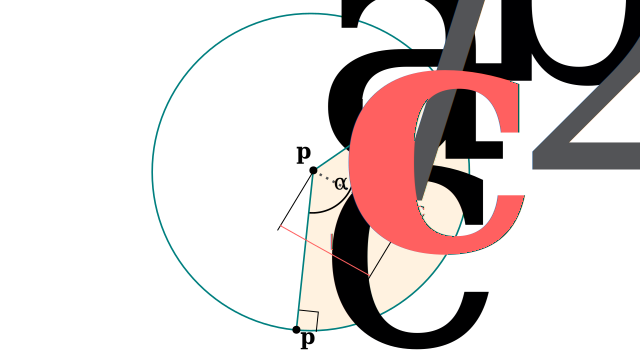
\includegraphics[width=0.6\linewidth]{figures/circleSector.png}}
	{\caption[A Circle Sector in Detail]{The circle sector produced by points $\bp_a$, $\bp_b$, and $\bp_c$, with $\alpha$ as the central angle bisected by a dotted line, and $\ell_{a,b}$ as the length between points $\bp_a$ and $\bp_b$ which is equal radius of the circle. Also labeled is the center of gravity $\bc$ as well as the distance from the center point $\bp_a$ to $\bc$, drawn in a coral color as $\check{\ell}$}\label{fig:circleSector}}
\end{figure}

%
%
%
\subsection{Topology}
\label{ch2sBssT}
Topology is the mathematical study of the properties of space that are preserved through deformations, twistings, and stretchings of objects\footnote{but not tearing or gluing}, which developed as a field of study from geometry and set theory through analysis of concepts such as space, dimension, and transformation. For example, a circle is topologically equivalent to an ellipse, because it can be deformed by stretching.~\cite{Weisstein19c} Of the major concepts, this thesis is most concerned with manifolds and neighborhoods.

%
\subsubsection{Manifolds}
A manifold is a topological space that is locally, but possibly not globally, Euclidean; a concept that is central to many parts of geometry because it allows complicated structures, such as the triangle mesh, to be described and understood in terms of the simpler, local topological properties. In general, that means that a manifold is an $n$D-subset of an Euclidean space $\mathbb{R}^{>n}$.~\cite[p.~199]{Mara12} For example, 1-dimensional manifolds in $\mathbb{R}^{2}$ include lines and circles, and 2-dimensional manifolds in $\mathbb{R}^{3}$, also called surfaces, can include commonly-known shapes such as the plane, the sphere, and the torus, but also of prime importance for this thesis, the triangle mesh.

%
\subsubsection{Neighborhoods}
A neighborhood is also one of the basic concepts of topology. Intuitively speaking, a neighborhood of a point is a set of points containing that point, where one can move in any direction without leaving the set. While determining the neighborhood is trivial for 1-dimensional manifolds, and relatively simple to regular surfaces, such as a 2D-images whose pixels have at most four neighbors in orthogonal directions with a geometric distance of 1, as well as four neighbors at the diagonal directions with a geometric distance of $\sqrt{2}$, determining the neighborhood becomes more complicated for irregular surfaces like those found in \tdd{}. With those surfaces, one must determine the set of neighbors using the associations that define the triangular faces; the details of which are covered in detail in Section:~\ref{ch2s3ssNRN}, after the necessary topics regarding \tdd{} have already been discussed.

Figure~\ref{fig:neighborhoods} illustrates in (a) and (b) the differences among one-ring neighborhoods in two kinds of regular meshes, a square mesh as in pixels of a digital image, and a triangle mesh, as in a hexagonal tessellation. Then in (c), the figure shows two very different one-ring neighborhoods in a single irregular triangle mesh typical of acquired \tdd{}. In particular, notice in (c) the completely arbitrary shape and size of the one-ring neighborhoods found in the irregular triangle mesh; even the number of neighbors varies widely. From this observation is where the motivation behind \fors{t} came.

\begin{figure}
\ffigbox
	{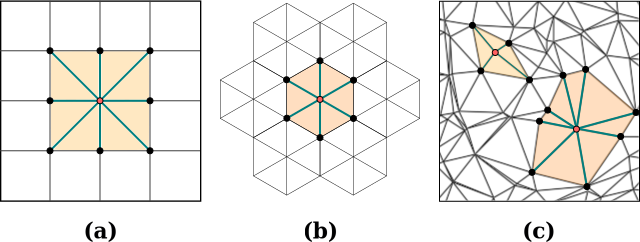
\includegraphics[width=1.0\linewidth]{figures/neighborhoods.png}}
	{\caption[One-ring neighborhoods in regular and irregular meshes]{One-ring neighborhoods in (a) a regular square mesh, as in pixels of a digital image (b) a regular triangle mesh, as in a hexagonal tessellation (c) an irregular triangle mesh, typical of acquired \tdd{}}\label{fig:neighborhoods}}
\end{figure}

%
%
%
%
\section{\tdd}
\label{ch2s3}
\todoStyle{the 3 in \tdd{} looks too small}
The data upon which one convolves \fors{t} is called \tdd\todoCitation{\tdd{} name origin, BB82 from Mara12}. As described in Section~\ref{ch2s3ssM}, \tdd{} consists primarily of a single mesh $\bM$, which is the superset of $\bP$, a set of points, and the set $\bT$ consisting of triangular faces, each to be covered in Sections~\ref{ch2s3ssP} and~\ref{ch2s3ssF} respectively. \tdd{} also comes in two distinct flavors depending on its origin: acquired or synthetic, as discussed in Section~\ref{ch2s3ssAVS3}. The data can also include a texture map and other various types of information stored as scalar or vector fields, as elaborated on in~\ref{ch2s3ssFV}.

%
%
%
\subsection{Points}
\label{ch2s3ssP}
A point $\bp$ is the most primitive element of \tdd{}. ``Point'' is the abbreviated form of ``measuring point'', and is also known in other fields of study as a vertex, or a position vector $\bR{3}$\todoCitation{other names for a point}. A point is defined by the 3-dimensional Cartesian coordinates $x$, $y$, and $z$, and in \tdd{}, points are generally unique and not required to be in any particular order. In this thesis, a point is addressed using several different subscripts, depending on the context.

Index $v$ is the globally unique index, with which we can define the set
%
\begin{equation}
	\bP := \left \{\:\bp_v \mid v \in \mathbb{N}, \;\text{and}\; 1\leq v \leq v_{max}\:\right \}
	\label{eq:defineSetOfPoints}
\end{equation}
%
where $v_{max}$ is the maximum index\footnote{Beginning indices with 1 is significant because of the discordant conventions between addressing the first element of a data structure with 0 in programming languages, such as C++ and python, versus addressing first elements with 1, as is the standard for mathematical literature. Because this thesis should indeed be considered mathematical literature, we will always start indices at 1, and only use index 0 for special cases. For example, $\bp_0$ is used in Chapter~\ref{ch4} to represent the center point of the one-ring neighborhood.} of points in the data, and is equivalent to the cardinality of the set of points $|\bP|$.%
\nomenclature[ea]{$\bP$}{the set of points $\bp$ in $\bM$}%
\nomenclature[eb]{$\bp_v$}{a specific point in $\bP$}%

Otherwise, when referencing to a point within a particular face or neighborhood, the three corners can be referenced indirectly as $\bp_i$\footnote{or generally as $\bp_a$, $\bp_b$, $\bp_c$ in the case of Equation~\ref{eq:defineEdgeLengthFace}, or in the case of a nested loops: as $\bp_i$ in Algorithm~\ref{alg:serialBuildNeighborhoods}, and $\bp_j$ in Algorithm~\ref{alg:serialCompute}}, $\bp_{\sipo}$, and $\bp_{\sipt}$, or directly as $\bp_1$, $\bp_2$, and $\bp_3$.~\cite[p.~25]{Mara12}%
\todoReword{ensure footnote indices remain correct}%
\nomenclature[ec]{$\bp_i$}{also $\bp_{\sipo}$, and $\bp_{\sipt}$; one of three indirectly referenced points comprising a face}%

%
%
%
\subsection{Faces}
\label{ch2s3ssF}
Faces are the another primitive element of \tdd{}. As we are working exclusively with triangular meshes~\cite[p.~26]{Mara12}, we define a face $\bt$ by the totally ordered~\cite{Weisstein19a} set of three distinct points, which we will index in clockwise order\footnote{It is worth mentioning here that many software packages, such as the GigaMesh Framework~\cite[p.~89]{Mara12}, may expect counter-clockwise ordering of indexes. This is significant because the ordering provides an orientation by which visualization software can apply texture and/or lighting. The only mathematical significance of the ordering is the sign of the area of a face, and totally inconsequential when the absolute value is expected, as shown by\cite[p.~2]{Braden86}. This is yet another example of the difference between the conventions of mathematical literature versus those of computer science. And again, because this thesis should indeed be considered mathematical literature, we will continue to follow the conventions of mathematical literature.}~\cite[p.~4]{Mara17}.
\todoResearch{does the "right-hand-rule apply here?"}
%
\begin{equation}
	\bt := \left \{\,\bp_a,\,\bp_b,\,\bp_c\right \} = \left \{\,\bp_1,\,\bp_2,\,\bp_3\right \}
	\label{eq:defineFaces}
\end{equation}

With the introduction of faces comes the concept of adjacency. A face $\bt_i$ is said to be adjacent to another face $\bt_j$ if, and only if, they share the same subset of two points. Similarly, a point $\bp_a$ is said to be adjacent to another point $\bp_b$ if, and only if, the set $\{\bp_a, \bp_b\}$ is a subset of at least one face $\bt \in \bT$. A synonym for adjacent is ``neighboring'', and this thesis will use both interchangeably. \todoReword{add equation for these identities}\todoReword{index entry for adjacent}

The Figure~\ref{fig:triangularFaces} shows two adjacent triangular faces $\bt_1$ and $\bt_2$, and the relationship between their points $\bp_a$, $\bp_b$, and $\bp_c$, their edge lengths $\ell_a$, $\ell_b$, and $\ell_c$, and their clockwise orientation.

\begin{figure}
\ffigbox
	{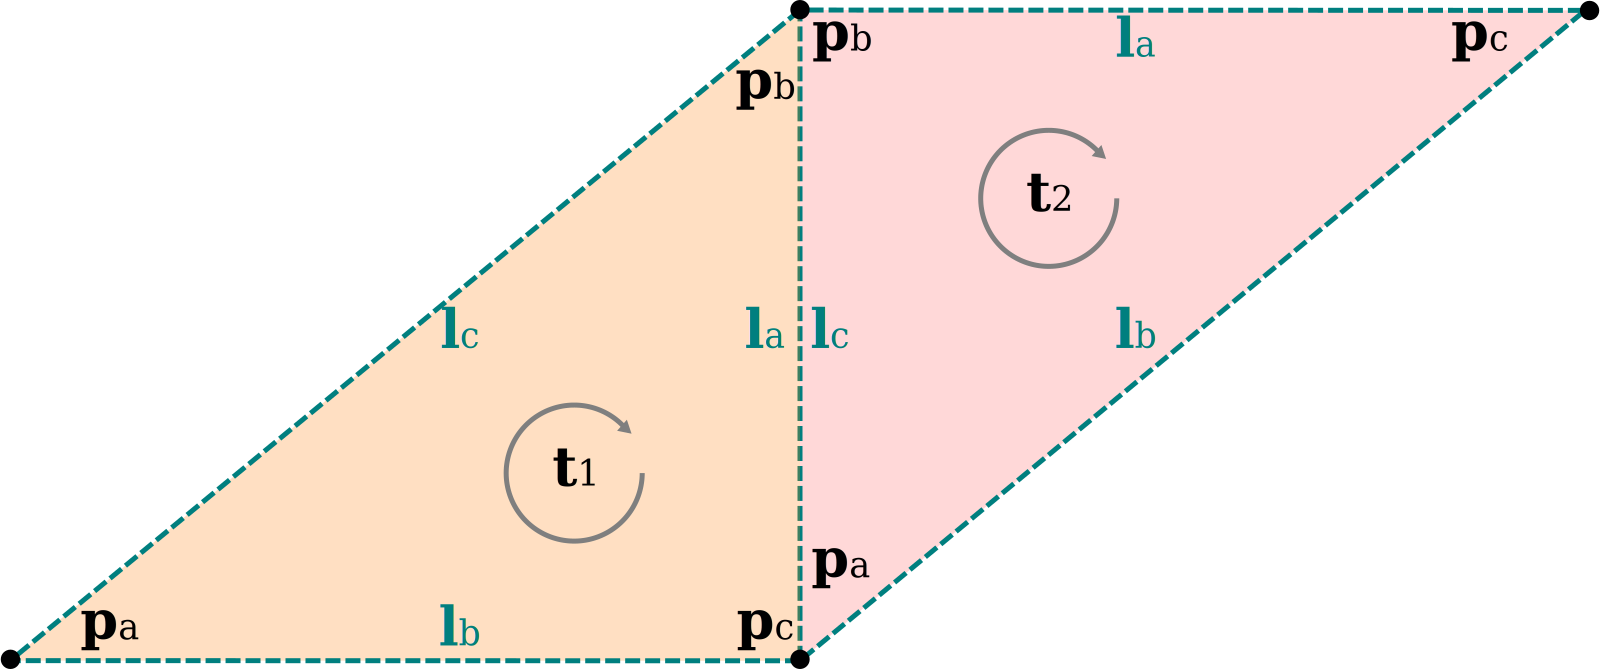
\includegraphics[width=1.0\linewidth]{figures/triangularFaces.png}}
	{\caption[Two Triangular Faces]{Two adjacent triangular faces $\bt_1$ and $\bt_2$, showing the relationship between their points $\bp_a$, $\bp_b$, and $\bp_c$, their edge lengths $\ell_a$, $\ell_b$, and $\ell_c$, and their clockwise orientation.}\label{fig:triangularFaces}}
\end{figure}

Each distinct triangular face is addressed using the global index $k$, and when taken together, comprise the family of sets
%
\begin{equation}
	\bT := \left \{\:\bt_k \mid k \in \mathbb{N}, \;\text{and}\; 1\leq k \leq k_{max}\:\right \}
	\label{eq:defineSetOfFaces}
\end{equation}
%
where $k_{max}$ is the maximum index of faces in the data, and is equivalent to the cardinality of the set of faces $|\bT|$.%
\nomenclature[fa]{$\bT$}{the set of faces $\bt$ in $\bM$}%
\nomenclature[fb]{$\bt_k$}{a specific face in $\bT$}%

%
%
%
\subsection{Edge Lengths}
\label{ch2s3ssEL}
As illustrated in Figure~\ref{fig:triangularFaces}, each triangular face is implicitly composed of three edges. Despite the fact that an edge is not typically\footnote{Other data structures, such as the Winged-Edge~\cite[p.~1]{Baumgart75}, may use edges as a primitive element} a primitive element of \tdd{}, we will endeavor to define the length of an edge $\ell$, because edge lengths are of particular significance for both the design and implementation of \fors{t}.

What is also particularly interesting about Figure~\ref{fig:triangularFaces}, is that when edge lengths are defined by the points of specific faces, each non-border edge length, illustrated by the figure as $\ell_a$ in $\bt_1$, and $\ell_c$ in $\bt_2$, will be labeled twice, despite representing the same distance.

When in the context of a particular face $\bt_k$, we will use a single index to define the length
%
\begin{equation}
	\ell_a := |\bp_b - \bp_c| \enspace:\enspace \left \{\,\bp_a,\,\bp_b,\,\bp_c\right \} = \bt_k
	\label{eq:defineEdgeLengthFace}
\end{equation}%
\nomenclature[ga]{$\ell_i$}{the length of the edge opposite the point $\bp_i$ of a specific face}%
%
and double indices when an edge length is referenced in relation to a specific point $\bp_v$ and its neighbor $\bp_i$
%
\begin{equation}
	\ell_{\sv{i}} := |\bp_i - \bp_v|
	\label{eq:defineEdgeLengthPoint}
\end{equation}%
\nomenclature[gb]{$\ell_{\sv{i}}$}{the length of the edge between points $\bp_v$ and $\bp_i$}%

Please note the similar notation for the cardinality of a set $|\bP|$, to that for the calculation for the length of the edge $|\bp_i - \bp_v|$ as defined in Equation~\ref{eq:defineEdgeLengthPoint}. While cardinality is simply the count of elements in the set, the length is calculated as the L2-norm of the referenced vector.~\cite[p.~26]{Mara12}

%\begin{align}
\begin{equation}
\begin{aligned}
	|\bp_i - \bp_v| & = \lVert\bp_i - \bp_v\rVert_2 \\
					& = \sqrt{(x_i-x_v)^2 + (y_i-y_v)^2 + (y_i-y_v)^2}
	\label{eq:defineEdgeLengthCalc}
\end{aligned}
\end{equation}
%\end{align}
\todoResearch{can I avoid sqrt altogether by performing entire algorithm squared?}

%
%
%
\subsection{Meshes}
\label{ch2s3ssM}
In \tdd{}, a mesh $\bM$ is the digital representation of a discrete manifold embedded in $\bR{3}$, and is typically\footnote{except in the case of specifically designed synthetic data~\ref{ch7sSD}} 2D-non-planar\todoStyle{in 2D, the 2 looks small} and comprised of non-regular, triangular faces composed of connected points.~\cite[p.~25]{Mara12} A mesh is the superset defined as
%
\begin{equation}
	\bM := \left \{\bP,\:\bT\right \}
	\label{eq:defineMesh}
\end{equation}%
\nomenclature[da]{$\bM$}{a mesh; the superset including the sets of all points $\bp$ and faces $\bt$}%
%
with the set $\bP$ consisting of points, and the set $\bT$ consisting of triangular faces.

Many 3D-scanners produce point clouds\todoCitation{3D-scanners produce point clouds}, which as the name suggests, are comprised soley of a set of points $\bP$ and do not provide the set $\bT$. However, it is possible, and necessary for the production of a mesh, to perform a point set triangulation\todoCitation{perform a point set triangulation} in order to connect $\bP$ into a set of triangle faces, enabling one to combine the two sets into a mesh.~\cite[p.~26]{Mara12} For example, during our experiments, we perform the well-known Delaunay triangulation\todoCitation{Delaunay triangulation} in order to produce a mesh from a randomly generated point cloud\todoReference{experiments}.

%
%
%
\subsection{One-ring Neighborhoods}
\label{ch2s3ssORN}
It was mentioned in Section~\ref{ch2sBssT}, that determining the neighborhood of a point $\bp_v$ is non-trivial. Having now examined the definitions of points, faces, and meshes, we can now formalize the one-ring neighborhood in \tdd{} as
%
\begin{equation}
	\bN_v := \left \{\;\bp_i\;|\;\left \{\,\bp_i,\,\bp_v\right \} \subseteq \bt \quad \forall \bt \in \bT\;\right \}
	\label{eq:defineNeighborhood}
\end{equation}%
\nomenclature[ha]{$\bN_v$}{the set of points comprising the one-ring neighborhood about $\bP_v$}%
\nomenclature[hb]{$\bp_i$}{a one-ring neighbor of $\bp_v$}%
%
which in words, means that the neighborhood $\bN_v$ is defined as the set of points $\bp_i$ such that both $\bp_i$ and $\bp_v$ are two points of a triangular face $\bt$, for all faces in the mesh.

When taken together, all the neighborhoods $\bN_v$ comprise a set of sets of neighbors; the family of sets $\bN$, with the common quality being that all the subsets are neighborhoods. The cardinality of each neighborhood $|\bN_v|$ will likely vary among other neighborhoods in $\bM$, however, the value and must always be $\geq 2$, and though there is no upper limit, $|\bN_v|$ is typically $\leq 12$. Furthermore, the neighboring points are always indexed in a clockwise direction for the same reasons as discussed in Section~\ref{ch2s3ssF}.
\nomenclature[hc]{$\bN$}{a family of sets of neighborhoods}%
\todoResearch{get real upper limit for n}.%

As illustrated in Figure~\ref{fig:neighborhoods}, the set of black points are the $\bp_i$ which belong to $\bN_v$, what is known as a one-ring neighborhood of $\bp_v$, because they are directly connected with the center point $\bp_v$ drawn in coral color. The moniker originates from graph theory where each adjacent point is said to have a relative distance of 1 within the graph\todoReword{do I need graph theory in basic theory section?} of the mesh. The one-ring can be extended to a 2-ring by taking the union of the neighborhood $\bN_v$ with each neighborhood of each one-ring neighbor $\bp_i$, which adds points having the relative distance of 2 within the graph. This iterative concept can be repeated k times and the neighborhood is than referred to as k-ring. Unfortunately, the relative distance within the graph can not be assumed equal to the geometric distance nor geodesic distance, regardless of that fact, it is used throughout the literature – especially in the field of Computer Graphics.~\cite[p.~29]{Mara12}

Our solution for computing \fors{t} in light of these complications is explained in greater detail in Chapter~\ref{ch4}, later in this thesis.
\todoReword{consider making a footnote}

%
%
%
\subsection{Acquired vs Synthetic \tdd{}}
\label{ch2s3ssAVS3}
The corpus of \tdd{} exists in two flavors, acquired and synthetic data, with each being handily classifiable by the fashion in which it was generated, and the characteristics innate to those techniques.\todoReword{consider adding a figure here showing difference, or referencing a figure or pair of figures that does}

Acquired \tdd{} is typically captured as a point cloud utilizing various methods, such as: LiDAR (Light Detection and Ranging), Structured Light, or Structure from Motion~\cite[p.~19]{Mara12}. Then the data is exported from software packages accompanying the 3D-scanners as either just the point cloud as a simple set of points $\bP$, or optionally as a triangle mesh $\bM$, described by one or more scalar-fields. Acquired \tdd{} also often consists upwards of a million points and as many as twice that number of faces\todoReference{the interesting experimental finding about face to vertex ratio; add as a footnote}. These exported meshes ~\cite[p.~25]{Mara12} uniformly contain noise and may exhibit other complexities for analysis, such as: non-manifold points, multiple borders and holes in the surface, inverted face orientation, non-manifold edges, and agglutination or degenerate faces. ~\cite[p.~28-32]{Mara12}

Conversely, synthetic \tdd{} is artfully crafted to obey the constraints of being a good mesh\todoReword{define a good mesh here}, without the complexities exhibited by acquired data. When modeling 3-dimensional objects, synthetic \tdd{} can require significantly less memory for storage, as simplifications can be made for large regular surfaces. For example, even the largest flat, rectangular surface can be modeled with only four points and two faces, whereas the acquired data methods require that the Nyquist–Shannon sampling theorem\todoCitation{Nyquist Shannon Theorem} be obeyed for the smallest detectable feature throughout the entire surface.~\cite[p.~19]{Mara12}~\cite[p.~3]{Mara17}

For our experiments\todoReference{experiments}, we created another kind of synthetic \tdd{} which does not model a 3D-object. Instead, these synthetic-mesh generators produce different types of tessellations on arbitrarily large, planar surfaces, accompanied by a configurable scalar-field of function values.

%
%
%
\subsection{Function Values}
\label{ch2s3ssFV}
In addition to the three Cartesian coordinates, a point may often contain other relevant data in the form of scalar fields, or when taken together, vector fields. This information, which is stored at each point $\bp$, often includes data regarding: RGB color, material type, reflectivity, transparency, quality, confidence, or the resulting function values from an analytical filter such as the Multi-Scale Integral Invariants (MSII) filter~\cite[p.~21]{Mara12}, but can be extended to include data important to other fields of study, such as: infrared or ultraviolet light, temperature, rainfall, population, crime-rates, etc; essentially, any kind of data that may be measured at a point. As \fors{t} will currently\todoReference{future work/applications} only process a single field at a time, we can define a scalar field simply as the set of function values
%
\begin{equation}
	\bF := \left \{\: f_v \mid v \in \mathbb{N}, \;\text{and}\; 1\leq v \leq v_{max} \:\right \}
	\label{eq:defineSetOfFunctionValues}
\end{equation}%
\nomenclature[ia]{$\bF$}{the set of function values $f$; a scalar field}%
\nomenclature[ib]{$f_v$}{a specific function value in $\bF$, corresponding to $\bp_v$}%
%
This definition shares the indices $v$ and $v_{max}$ with the definition for a set of points, Equation~\ref{eq:defineSetOfPoints}. Indeed, it is a fact that the cardinality of $|\bF|$ must be equal to $|\bP|$
%
\begin{equation}
	|\bF| \mbeq |\bP|
\end{equation}
%
because function values are only stored alongside the Cartesian coordinates, 1-for-1 with points, due to \tdd{} existing as a discrete manifold.\todoResearch{storing data between points on a discrete manifold}

%
%
%
%
%
\section{Parallel Processing}
\label{ch2sPP}

%
\subsection{Architectures of Concurrency}
Hardware consists of memory and processors. Memory is divided into a hierarchy which starting at the registers on the processors themselves, increases in capacity, but decreases in speed.\todoReword{moves away from} Of particular interest to this thesis...\todoReword{continue}

%
\subsection{Concurrency vs Parallelism}
\label{ch2sACssCVP}

%
\subsection{Flynn's taxonomy}
1.1	Single instruction stream single data stream (SISD)
1.2	Single instruction stream, multiple data streams (SIMD)
1.3	Multiple instruction streams, single data stream (MISD)
1.4	Multiple instruction streams, multiple data streams (MIMD)

\subsubsection{SIMT Architecture}%4.1. SIMT Architecture}
%
\subsection{Critical Sections}
\label{ch2sPPssCS}
Thread Safety. C++ STL is not thread safe!

%
\subsection{Mutexes and semaphores (binary semaphore}
\label{ch2sPPssMS}
While it is true that any locking mechanism can be expensive to both compute time and memory, \todoResearch{how expensive are locking mechanisms} typically, with acquired \tdd{}, the ratio of points in $\bP$ to the average neighborhood size \todoReword{add symbol for average neighborhood size} approaches $|\bP|$, therefore the speedup gained by exploiting the concurrency is definitely\todoResearch{quantify the cost} worth the cost of the added synchronization overhead when computing with even moderately sized meshes on a SIMP or SIMT modeled architecture.
starts at ~\cite[~p.20]{Lang17}

%
\subsection{Control \& Data Dependencies}
\todoResearch{https://en.wikipedia.org/wiki/Loop-level\_parallelism}
%True (Flow) Dependence	S1 ->T S2	A true dependence between S1 and S2 means that S1 writes to a location later read from by S2
%Anti Dependence	S1 ->A S2	An anti-dependence between S1 and S2 means that S1 reads from a location later written to by S2.
%Output Dependence	S1 ->O S2	An output dependence between S1 and S2 means that S1 and S2 write to the same location.
%Input Dependence	S1 ->I S2	An input dependence between S1 and S2 means that S1 and S2 read from the same location.
The concepts of control and data dependencies are not new ones, and can be dated back to the invention of multi-pass compilers\todoCitation{Data Dependencies and multi-pass compilers}. The field of study regarding the details is called dependence analysis and has far-reaching consequences from business management, economics, as well as software optimization\todoCitation{dependence analysis}. In general, the basic concept behind both control and data dependencies is that some procedure A is said to be dependent on another procedure B, if A requires B to be executed first.

Figure~\ref{fig:simpleControlDependency} shows the ubiquitous if-then control structure as a simple example of a control dependency. It reads, ``if B is true, then do A''. In this case A is control dependent on B, because B must execute before it can be determined wether or not to execute A.

\tikzset{%
	>={Latex[width=2mm,length=2mm]},
	base/.style = {rectangle, rounded corners,
		draw=black, thick,
		minimum width=1cm, minimum height=1cm,
		text centered, font=\sffamily},
	operation/.style = {base, draw=MyTeal, fill=MyLtTeal},
	halt/.style = {base, draw=MyCoral, fill=MyLtCoral}
}
\begin{figure}[ht]
\centering
\ffigbox{
	\begin{tikzpicture}[node distance=1.2cm, every node/.style={fill=white, font=\sffamily}, align=center]
		\node (ifB) [operation] {if $B$};
		\node (doA) [operation, right of=ifB, xshift=2cm] {do $A$};
		\node (stop) [halt, below of=doA] {$stop.$};

		\draw[->] (ifB) -- (doA) node[pos=.5]{true};
		\draw[->] (ifB) .. controls +(down:1cm) and +(left:1cm) .. (stop) node[pos=.5]{false};
	\end{tikzpicture}}
	{\caption[If-Then Control Dependency]{A simple example of control dependency using the if-then control structure, with each distinct operation colored in teal, and control dependency marked with an arrow.}\label{fig:simpleControlDependency}}
\end{figure}

Figure~\ref{fig:dataDependencyOfL2Norm} illustrates the less-than-simple example of data dependencies inherent to calculating the L2-norm of a position vector in $\mathbb{R}^{3}$, which has already been seen in Equation~\ref{eq:l2norm}, and will be seen often in this thesis. There are six individual procedures involved with calculating the L2-norm: three squarings, two additions, and one square root. The three squaring procedures are totally independent of each other and can be performed in any order, indeed even concurrently, in relation to one another. In contrast, the two additions are totally dependent on their addends. While the order in which the first two of the three addends are used is inconsequential, the first addition is always dependent on the completion of two squarings, and the second addition is dependent on not only the sum from the first addition, but the product of the third squaring as well. Finally, because the square root procedure is dependent on the execution of both additions, it also inherits their dependencies on the squaring procedures, and therefore must wait until the very end before executing last.\todoResearch{name of this inheritance, associative?}

\tikzset{%
	>={Latex[width=2mm,length=2mm]},
	base/.style = {rectangle, rounded corners,
		draw=black, thick,
		minimum width=1cm, minimum height=1cm,
		text centered, font=\sffamily},
	operation/.style = {base, draw=MyTeal, fill=MyLtTeal},
	bigBlock/.style = {base, draw=MySand, fill=MyLtSand},
		smOr/.style = {fill=MyLtSand},
}
\begin{figure}[ht]
\ffigbox{
	\begin{tikzpicture}[node distance=1.25cm, every node/.style={fill=white, font=\sffamily}, align=center]
		\node (xx1) [operation] {$x\cdot x$};
		\node (yy1) [operation, below of=xx1] {$y\cdot y$};
		\node (zz1) [operation, below of=yy1] {$z\cdot z$};
		%\coordinate (join1) at ([xshift=2.0cm]yy1.east);
		\node (adds) [bigBlock, right of=yy1, xshift=4cm, minimum width=3.5cm, minimum height=4.725cm] {};
			\node (xxpyy) [operation, below=(.125cm of adds.north), xshift=-.85cm] {$x^2 + y^2$};
			\node (zz2) [operation, right=(.75cm of xxpyy)] {$+\,z^2$};

			\node (or1) [smOr, below=(.125cm of xxpyy), xshift=1cm] {-xor-};

			\node (yypzz) [operation, below=(.125cm of or1), xshift=-1cm] {$y^2 + z^2$};
			\node (xx2) [operation, right=(.75cm of yypzz)] {$+\,x^2$};

			\node (or2) [smOr, below=(.125cm of yypzz), xshift=1cm] {-xor-};

			\node (zzpxx) [operation, below=(.125cm of or2), xshift=-1cm] {$z^2 + x^2$};
			\node (yy2) [operation, right=(.75cm of zzpxx)] {$+\,y^2$};
		\node (sqrtAll) [operation, right of=adds, xshift=4cm] {$\sqrt{x^2+y^2+z^2}$};

		\draw[->] (xx1) -- (adds);
		\draw[->] (yy1) -- (adds);
		\draw[->] (zz1) -- (adds);
		%\draw[-] (xx1) -- (join1);
		%\draw[-] (yy1) -- (join1);
		%\draw[-] (zz1) -- (join1);
		%\draw[->] (join1) -- (adds);
		\draw[->] (xxpyy) -- (zz2);
		\draw[->] (yypzz) -- (xx2);
		\draw[->] (zzpxx) -- (yy2);
		\draw[->] (adds) -- (sqrtAll);
	\end{tikzpicture}}
	{\caption[Data Dependencies in the L2-norm Calculation]{The data dependencies inherent to calculation of the L2-norm of a position vector in $\bR{3}$, with each distinct operation colored in teal, and data dependencies marked with arrows. The centered block in sand color represents an exclusive-or situation, abbreviated as xor, where one, and only one pair of operations shall execute.}\label{fig:dataDependencyOfL2Norm}}
\end{figure}

%
%Data Partitioning:
%Calculations depend on specific data structures.~\cite[p.~357]{Lang17}
%As in edge lengths depend on the neighborhoods.

%
%Data Dependencies: ~\cite[p.~358]{Lang17}
%Section~\ref{ch2sACssCVP}
%
%Functional Partitioning: ~\cite[p.~359]{Lang17}
%different operations on the same data

%
\subsection{Serial Computation \& Threads}
In a very general sense, when a computer executes a serial program, it proceeds one instruction at a time, sequentially in the order that it is written, reading and writing to memory as required. Individually, these are called threads of execution, and a single processing core can only process a single such thread at a time, however, it can rapidly perform context switching\todoCitation{context switching} among a multitude of self-contained threads, each with their own unique ids and memory addresses, in order to give the illusion of parallel processing.

As memory to be processed by a thread is stored somewhere in a hierarchy which increases in size, but decreases in speed as one moves from the processor's registers, it is likely that a context switch will cause what is known as a cache miss\todoCitation{cache hit or miss, check Lang}, which incurs a time penalty while the processing stalls and the required memory is read from slower hardware sources.

\todoBackground{"spawning a thread"}

%
\subsection{Multi-threaded Computation}
All modern computers implement some form of parallelism, be it multi-core or multi-threaded processors, stream processors as found in GPUs, or networks of supercomputers or data centers. This thesis will focus on implementing \fors{t} in a way which can utilize the parallelism provided by the array of stream processors found in a commercially available GPGPU.
\todoBackground{synchronizeThreads()}
\todoBackground{memory vs speed}
\subsubsection{Explicit Synchronization}%3.2.5.5.3. Explicit Synchronization}
%
\subsection{Hardware Implementation}%4. Hardware Implementation}
%
%
%
%\section{CUDA extended C++: An interface for GPGPU implementation}

%
%
%
%\subsection{The C++ Standard Library}

%
%\subsubsection{Set}
%\label{ch2sCECssCSLsssS}
%\todoCitation{https://en.cppreference.com/w/cpp/container/set}

%\subsection{CUDA C Runtime}%3.2. CUDA C Runtime}

%\subsection{Versioning and Compatibility}%3.3. Versioning and Compatibility}
%\subsection{Host Memory and Device Memory}
%\subsection{Versions <9, vs >= 9}
%
%
%
%
%
%\section{Evaluation and Analysis of Concurrent Algorithms}~\cite[p.~330]{Lang17}
%Multi-node out of scope?!
%
\subsection{Timing}
%\begin{equation}
%	N = input size (num. ops)
%	P = processor count
%	Ts(N) = Sequential execution time
%	Tbest(N) = Optimal execution time
%	TP(N, P) = Parallel runtime
%\end{equation}
%
\subsection{Speedup, efficiency}
%	Speedup:
%S(N, P) = Tbest(N)/TP(N, P)

%	Efficiency:
%E(N, P) = Tbest (N)/PTP(N, P) = S/P

%	Costs:
%C(N, P) = PTP(N, P)
%
\subsection{Degree of Parallelism}
%	0 < q < 1 is the sequential part
%	1-q = is the parallelizable part
%
\subsection{Iso-efficiency}
%	WK(P) = iso-efficient if it fulfills:
%	TO(WK(P), P) = KWK(P)~\cite[p.~350]{Lang17}
%
\subsection{Scalability}
%	A parallel system is called scalable only if in has an iso-efficency function
%
%
%
%
%
\section{Summary}
%
